% Copyright 2021  Ed Bueler

\documentclass[10pt,hyperref,dvipsnames]{beamer}

\mode<presentation>{
  \usetheme{Madrid}
  \usecolortheme{beaver}
  \setbeamercovered{transparent}
  \setbeamerfont{frametitle}{size=\large}
}

\setbeamercolor*{block title}{bg=red!10}
\setbeamercolor*{block body}{bg=red!5}

\usepackage[english]{babel}
\usepackage[latin1]{inputenc}
\usepackage{times}
\usepackage[T1]{fontenc}
% Or whatever. Note that the encoding and the font should match. If T1
% does not look nice, try deleting the line with the fontenc.

\usepackage{empheq}
\usepackage{xspace}
\usepackage{verbatim,fancyvrb}

\usepackage{tikz}
\usetikzlibrary{shapes,arrows.meta,decorations.markings,decorations.pathreplacing,fadings,positioning}

\usepackage{hyperref}

% If you wish to uncover everything in a step-wise fashion, uncomment
% the following command:
%\beamerdefaultoverlayspecification{<+->}

\newcommand{\ba}{\mathbf{a}}
\newcommand{\bb}{\mathbf{b}}
\newcommand{\bc}{\mathbf{c}}
\newcommand{\bbf}{\mathbf{f}}
\newcommand{\bg}{\mathbf{g}}
\newcommand{\bn}{\mathbf{n}}
\newcommand{\bq}{\mathbf{q}}
\newcommand{\br}{\mathbf{r}}
\newcommand{\bx}{\mathbf{x}}
\newcommand{\by}{\mathbf{y}}
\newcommand{\bv}{\mathbf{v}}
\newcommand{\bu}{\mathbf{u}}
\newcommand{\bw}{\mathbf{w}}

\newcommand{\bF}{\mathbf{F}}
\newcommand{\bG}{\mathbf{G}}
\newcommand{\bQ}{\mathbf{Q}}

\newcommand{\grad}{\nabla}
\newcommand{\Div}{\nabla\cdot}
\newcommand{\minmod}{\operatorname{minmod}}

\newcommand{\CC}{\mathbb{C}}
\newcommand{\RR}{\mathbb{R}}

\newcommand{\ddt}[1]{\ensuremath{\frac{\partial #1}{\partial t}}}
\newcommand{\ddx}[1]{\ensuremath{\frac{\partial #1}{\partial x}}}
\newcommand{\Matlab}{\textsc{Matlab}\xspace}
\newcommand{\Octave}{\textsc{Octave}\xspace}
\newcommand{\eps}{\epsilon}

\newcommand{\ip}[2]{\left<#1,#2\right>}

\newcommand{\xiphalf}{{x_{i+\frac{1}{2}}}}
\newcommand{\ximhalf}{{x_{i-\frac{1}{2}}}}
\newcommand{\Fiphalf}{{F_{i+\frac{1}{2}}}}
\newcommand{\Fimhalf}{{F_{i-\frac{1}{2}}}}
\newcommand{\Fiphalfn}{{F^n_{i+\frac{1}{2}}}}
\newcommand{\Fimhalfn}{{F^n_{i-\frac{1}{2}}}}

\newcommand{\trefcolumn}[1]{\begin{bmatrix} \phantom{x} \\ #1 \\ \phantom{x} \end{bmatrix}}
\newcommand{\trefmatrixtwo}[2]{\left[\begin{array}{c|c|c} & & \\ #1 & \dots & #2 \\ & & \end{array}\right]}
\newcommand{\trefmatrixthree}[3]{\left[\begin{array}{c|c|c|c} & & & \\ #1 & #2 & \dots & #3 \\ & & & \end{array}\right]}
\newcommand{\trefmatrixgroups}[4]{\left[\begin{array}{c|c|c|c|c|c} & & & & & \\ #1 & \dots & #2 & #3 & \dots & #4 \\ & & & & & \end{array}\right]}

\newcommand{\blocktwo}[4]{\left[\begin{array}{c|c} #1 & #2 \\ \hline #3 & #4 \end{array}\right]}

\newcommand{\bqed}{{\color{blue}\qed}}
\newcommand{\ds}{\displaystyle}

\newcommand\mynum[1]{{\renewcommand{\insertenumlabel}{#1}%
      \usebeamertemplate{enumerate item} \,}}


\title{Stokes problems using Firedrake}

\subtitle{A tutorial in stages for glaciologists}

\author{Ed Bueler}

\institute[UAF]{University of Alaska Fairbanks}

\date{April 2021}

%% this nonsense needed to start section counter at 0; see
%% https://tex.stackexchange.com/questions/170222/change-the-numbering-in-beamers-table-of-content
%\makeatletter
%\patchcmd{\beamer@sectionintoc}
%  {\ifnum\beamer@tempcount>0}
%  {\ifnum\beamer@tempcount>-1}
%  {}
%  {}
%\beamer@tocsectionnumber=-1
%\makeatother


\begin{document}
\beamertemplatenavigationsymbolsempty

\begin{frame}
  \maketitle
\end{frame}

\begin{frame}
  \frametitle{Outline}
  \tableofcontents[hideallsubsections]
\end{frame}


\section{the problem, and the equations}

\begin{frame}{fluid equations}

\begin{itemize}
\item FIXME
\end{itemize}
\end{frame}


\begin{frame}{the Stokes equations}

\hfill 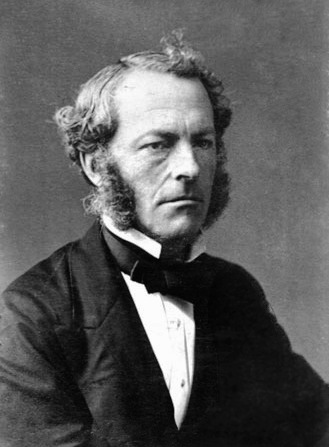
\includegraphics[width=0.25\textwidth]{figs/gstokes.jpg}

\vspace{-20mm}
\begin{itemize}
\item FIXME
\end{itemize}
\end{frame}


\section{stage 1: simple geometry, linear Stokes}

\begin{frame}{matrix for Stokes}

\begin{itemize}
\item simplest possible solver for linear stokes is direct method
\item FIXME
\begin{center}
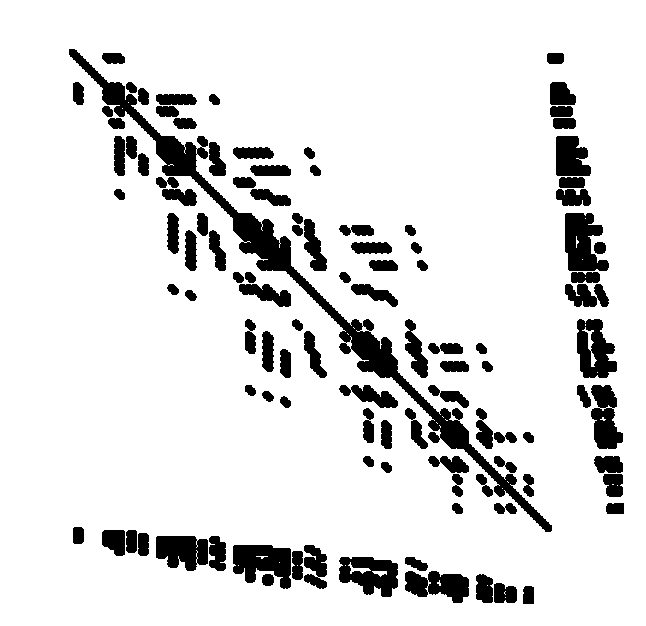
\includegraphics[width=0.5\textwidth]{figs/Kstokes.pdf}
\end{center}
\end{itemize}
\end{frame}


\section{stage 2: profile geometry, Glen-law Stokes}

\begin{frame}{Newton's method}

\hfill 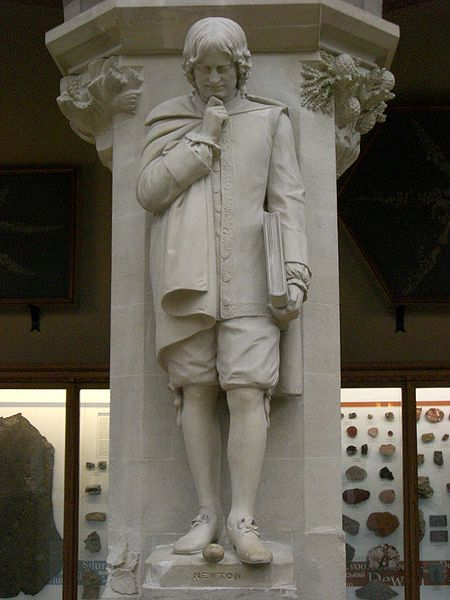
\includegraphics[width=0.25\textwidth]{figs/inewton.jpg}

\vspace{-20mm}
\begin{itemize}
\item FIXME
\end{itemize}
\end{frame}


\begin{frame}{FIXME}

\begin{itemize}
\item FIXME
\end{itemize}
\end{frame}


\section{stage 3: alternative extruded meshes}


\section{stage 4: solving faster and finer}

\begin{frame}{iterative linear methods}

\hfill 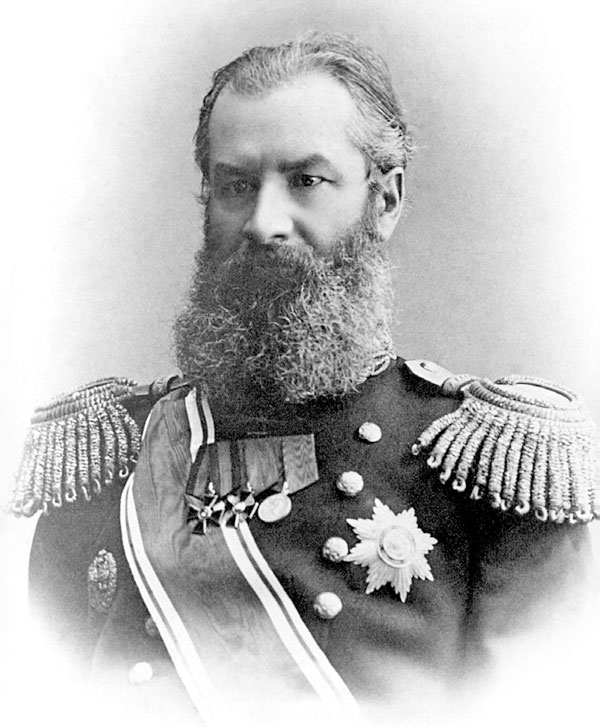
\includegraphics[width=0.25\textwidth]{figs/akrylov.jpg}

\vspace{-20mm}
\begin{itemize}
\item FIXME
\end{itemize}
\end{frame}

\begin{frame}{multigrid}

\begin{itemize}
\item FIXME
\end{itemize}
\end{frame}


\section{stage 5: 3D}

\begin{frame}{references}
\begin{columns}

\begin{column}{0.6\textwidth}
\begin{itemize}
\item Firedrake website
\item PETSc website
\item Elman
\item E.~Bueler, \emph{PETSc for Partial Differential Equations: Numerical Solutions in C and Python}, SIAM Press, 2021
\end{itemize}
\end{column}

\begin{column}{0.4\textwidth}

\includegraphics[width=\textwidth]{figs/firedrakebanner.png}

\bigskip
\hfill 
\includegraphics[width=0.8\textwidth]{figs/petscbanner.png}

\bigskip
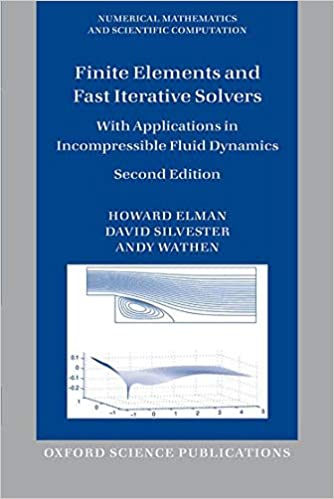
\includegraphics[width=0.42\textwidth]{figs/elmancover.jpg} \quad  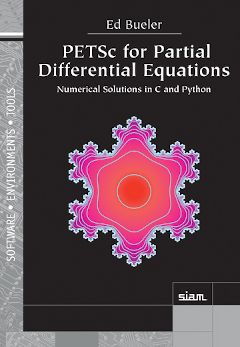
\includegraphics[width=0.44\textwidth]{figs/frontcover.jpg}
\end{column}

\end{columns}
\end{frame}


\end{document}
